\documentclass[conference]{IEEEtran}
\usepackage[justification=centering]{caption}
\usepackage{blindtext, graphicx}
\usepackage{float}

\begin{document}
\title{Three Approaches to a Team Building Application}

\author{\IEEEauthorblockN{Michael Goff\IEEEauthorrefmark{1},
Shashank Jha\IEEEauthorrefmark{2},
Jingjuan Deng\IEEEauthorrefmark{3} and
Bhaskar Sinha\IEEEauthorrefmark{4}}
\IEEEauthorblockA{Department of Computer Science, North Carolina State University, \\
Raleigh, North Carolina 27606\\ 
Email: \IEEEauthorrefmark{1}magoff2@ncsu.edu \\
\IEEEauthorrefmark{2}sjha5@ncsu.edu \\
\IEEEauthorrefmark{3}jdeng8@ncsu.edu \\
\IEEEauthorrefmark{4}bsinha@ncsu.edu}}


% make the title area
\maketitle

\section{Introduction}
The problem our team was looking to resolve was team creation in a classroom environment. Each of our group members has experiences a struggle with team situations in the past. Our surveys agreed with out predictions in that there are often problems in team building that relate to missing expertise and poor communication. To resolve these poor group situations, our applications will focus on creating teams with a wide variety of skill-sets to try to prevent a team from having an concentration of one skill and not have any members with knowledge of other required skills. Our first approach was an application that allowed for users to put up postings for a specific project and search for other users who fit the skill-set they require. The second approach focuses on a professor who would like to build a team with a wide breadth of skills without much effort on their part. The third application uses a weighted lottery to assign members to known projects based on how well they match up with the projects in question and their preferences for projects. 

For the design of our applications we decided to focus on using the Angular2 web framework and Firebase for our user management and data storage. We decided on these technologies because of their ease of use and the ability to abstract away a lot of the extra processes that do not pertain to our desired functionality like authentication systems. By using the same technologies for all three approaches we also hoped to enable the use of code reuse throughout the projects. 

\section{Approach 1}
In this approach we are looking at the problem for team creation from a student's perspective. According to our survey, on an average a student would do three to five projects during a semester, most of which are group projects. So with this approach we are making a web application in which the students of the class can log on and enter their skills. The skills would then be saved into the database along with the contact details of that student. Afterwards, the student can go on to the search page of the website and search for a particular skill (a skill which would be required while doing the project) which would return a list of all the students and their contact information present in the database, who possess that skill. Then with the contact information of those students, the student can get in touch with any of them to form a group. This approach is based on the idea that to do any project a variety of skills are required and if the user can find out different people with those skills it would enable the user to complete the project in a more effective way.

\subsection{Application Outline}
The front end of the web application uses AngularJS whereas the back end uses Firebase. The user is presented with a log in screen where they can sign up with a valid email address, if they are a new user, or log in with valid credentials, if they are an existing user. After log in, the user can add or remove skills and also edit their contact information. If the user is looking to make a team they can navigate to the search page and enter the skill in the search bar and the application will list out all the users in the database who possess that skill. The user can now go on and contact students with the contact information listed on the web page.

\subsection{Roadblocks}
Initially, the approach dealt with searching for people with a number of skills and not just one skill. This would have enabled the user to search for potential teammate with a number of skills and not just one skill. But, at the time of implementation this could not be achieved so instead we tweaked the approach to focus on just one skill. So, that the user could log onto the application and search for a person with a particular skill.

\section{Approach 2}
Unlike the other approaches, the second approach focuses on a professor's perspective when creating teams. This web application allows for a class to each log on and select their skills, and when all members have signed up a professor can select the create teams button. Teams will be formed based on the available skill sets in order to optimize the spread of skills across the teams. 

\subsection{Application Outline}
Creating the views was straight forward and we opted to make the pages simple for now to illustrate the functionality without wasting time on additional bells and whistles. Part of the focus on functionality was to ignore the need for a role based system between professors and students. We felt that using time to develop roles would take away from our time to focus on the important aspect of the application, building teams. As a result, our homepage features a list of all registered users and a check box grid of their skills, shown in figure \ref{home}. This will provide an indication of who will eventually be sorted into teams. On the header bar there is a button to generate teams. When clicked, the page will reload into a team view and present each team in a separate table. It will show the users' name, email, and skill-set. As for authentication we are using Firebase's built in system. We allow users to sign in either via Google in order to take advantage of their NCSU accounts or via the traditional email and password, as shown in figure \ref{login}. Due to the built in authentication we did not have to worry about storing sensitive user account info like passwords. Using the Firebase No-SQL database, we store each user's name, email and skills in user objects that are nested in a user list. We also have teams stored in a similar manner once they are created. 


\begin{figure}[H]
    \centering
    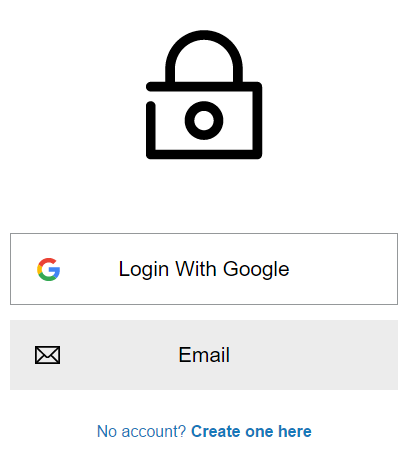
\includegraphics[width=5cm]{image/login.PNG}
    \caption{The Log-in Screen}
    \label{login}
\end{figure}

Overall, most of the functionality in this approach was on background implementation, since the functionality focused on automating the professor's task of team creation. As a result the front end is more limited regarding interactions for students. All they need to do is log in to the application in order to register themselves as a member of the team sorting pool. The professor just has to hit one button to create the teams, which are then listed on the page.

\subsection{Roadblocks}

One of the early struggles for the second approach was the framework we chose and some time-line stresses. The original plan was to reuse code from the first approach like the log-in feature in order to have a proper base for the second approach. However, when the time came it was determined to be easier to just use the Angular Command Line Interface (CLI) to create a new Angular2 project and plug into a Firebase environment with a package called AngularFire2. Using the CLI to create new components for the project was as simple as one command and it would automatically fill in all the boilerplate surrounding the project, allowing us to focus on the important aspects of development. 

\begin{figure}[H]
  \centering
  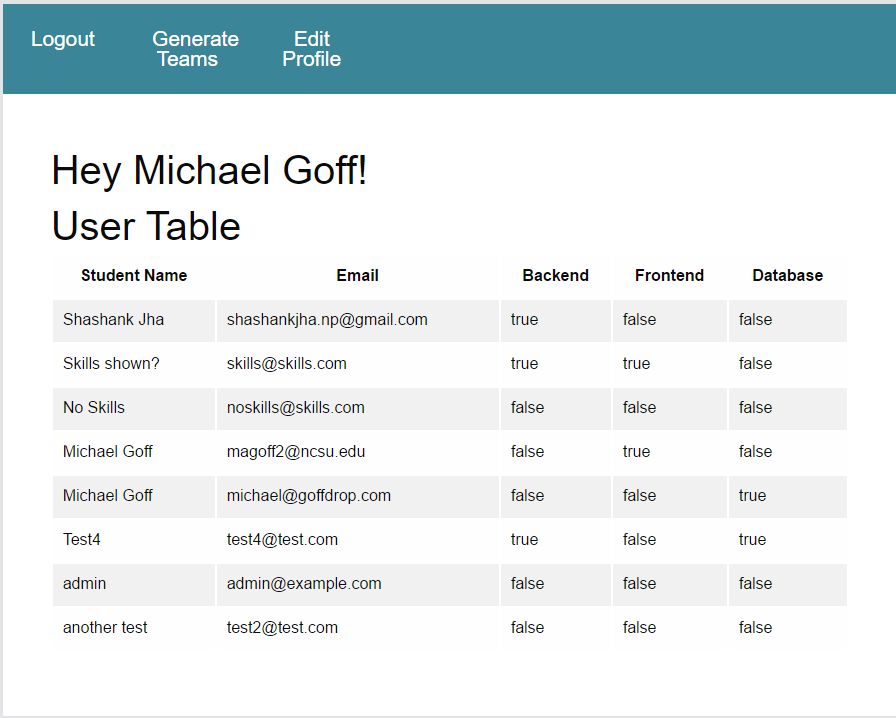
\includegraphics[width=6cm]{image/home.PNG}
  \caption{Team table}
  \label{home}
\end{figure}

There were a few additional development snags along the way when writing the second approach. One issue was to figure out how to collect the skills of a new user who authenticated through Google since abstracting authentication away led to confusion on whether or not a user was new. We have resolved this issue by redirecting Google users to a skills page to allow them to modify their skills upon logging in for the first time. This has also enabled us to add a link to allow users to edit their skills as well. Another issue was getting all of the data to appear in the tables throughout the application. After searching around online, we found that having incomplete data objects could lead to an error when querying for data. In order to error check for this kind of issue we found that if you add a question mark to the references it will do a safe look-up and if the object is not found, will just substitute blank data instead. 

One of the major function which is yet to implemented and tested is how to generate teams evenly. Even though we have rough idea of implementation, testing it for all corner cases will be tough. However since our target is not to make a perfect working algorithm, we should be able to complete it well within the deadline. A preliminary look at how the teams will be laid out can be seen in figure \ref{teampage}.

\begin{figure}[H]
  \centering
  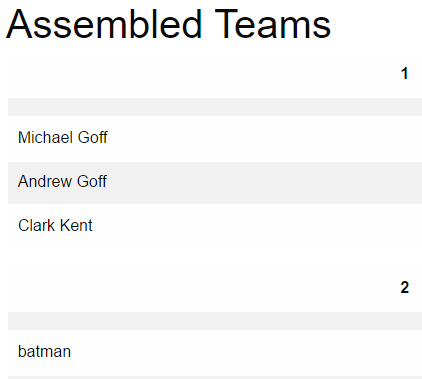
\includegraphics[width=6cm]{image/teams.PNG}
  \caption{Teams table}
  \label{teampage}
\end{figure}

The roadblocks for approach 2 were minimal in nature. There were not really any show stopping bugs that came as a result of development so it was a smooth process to create this application. Using the Angular CLI was a great way to avoid working on adding extra boilerplate code to our project manually and allowed us to focus on the important parts of the application. Having Firebase to abstract away a lot of the hassle of data management was a huge time-saver and was a valuable tool in sticking to our time-line. 

\section{Approach 3}
Originally we designed approach 3 as a lottery algorithm considering users' preferences and skills, which satisfy both teams and users' requirements. However, when implementing it, we found it difficult to determine preference, weight and other parameters in lottery and the implementation time cost was too high. Considering the time limit, we came up with another approach. The main design is that users can join a team whose positions are available and fit for users' skills. It's implemented as a web application based on JavaScript and HTML, with the support of a Firebase data server.

\subsection{Application Outline}
The new approach 3 is widely used, similar to the course selection process in college. The positions in a team is limited, so if one team is full, users have to choose other teams. This algorithm gives users freedom to choose their teams and teammates. Users must satisfy the skill requirement of specific position, to ensure building skill balanced teams.

Figure \ref{teams} shows a view in which user can choose one team to join. Positions do not match users skills or is occupied by other users are not available. Once joining a team, users can checkout the details of team members and connect with each other with information provided(Figure \ref{team_info}). If a user is not satisfied with the team formation, she/he can quit the current team and join another one.

\begin{figure}[H]
  \centering
  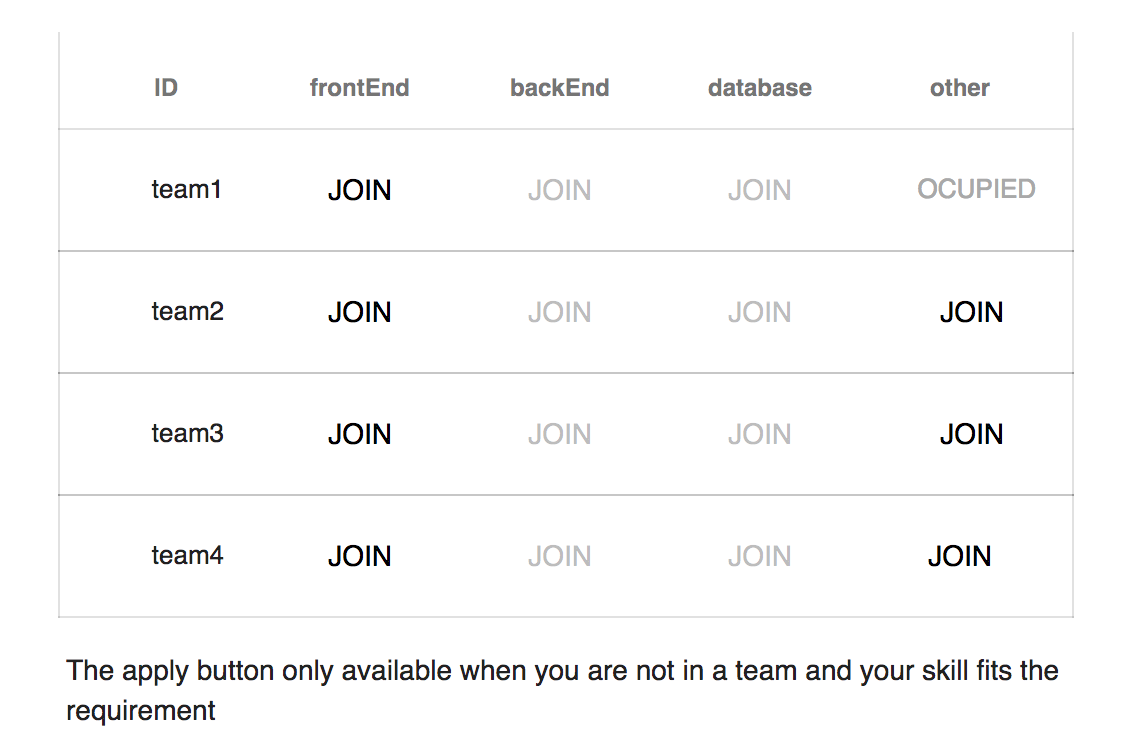
\includegraphics[width=6cm,height=4cm]{image/app3-teams.png}
  \caption{Team table}
  \label{teams}
\end{figure}
\begin{figure}[H]
  \centering
  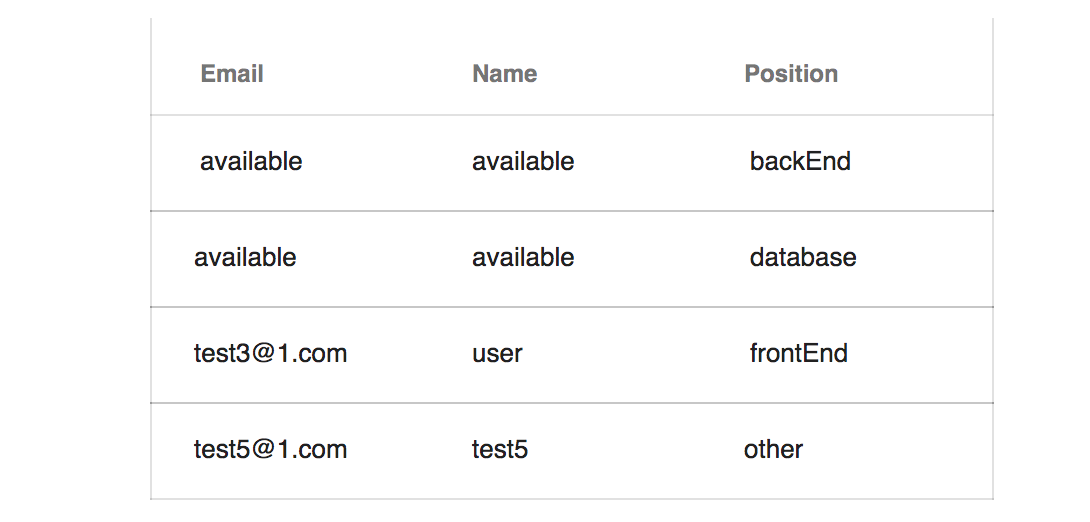
\includegraphics[width=6cm,height=3cm]{image/app3-teaminfo.png}
  \caption{Team table}
  \label{team_info}
\end{figure}

\subsection{Roadblocks}
During the development of approach 3, we met three major problems: nested data design, data synchronization and testing.

Data structure design

We have to record positions and team members, in addition to keeping track of which team users have joined. There are three structure of this relation, the first is recording keys in both data object, the second is build relational data, the third is recording relations only in one object(team or user) then tracking other objects by the keys. In approach 3, the first one is chosen. Although this data structure will have some redundancy, adding keys in both objects can reduce nested data retrieving. Consider the primary users of this app are usually in class or department size but not a large population, we trade off some space for shorter data accessing time and easy implementation.

Synchronization

Approach3 faced a problem of data synchronization. This problem occurred when A user quit a team, the user was not in a team but the team information still hadn't been updated. As a result the position is still unavailable to other users. Another scenario was when two users applied for the same position, only one of them was recorded in team object, but the team was recorded in both users' information. These kind of bugs due to Firebase asynchronous data stream. To solve these problem, we use synchronized function to execute code in sequence, and add rollback mechanism when the previous action fails.

Testing

There are different kinds of tools used to test JavaScript code. But some of them do not support testing external service such as Firebase. Since approach 3 is largely based on data server, testing with Firebase support is required. The possible solution is implementing the code in a new language such as Angular-CLI instead of normal JavaScript, which support many external libraries and servers.

\section{Conclusion}
In conclusion, all the three approaches attempt to solve the problem statement in three different ways. Approach one works from a student's perspective and enables the student to find out potential team mates based on the skills which would be needed to make the project. Whereas, approach two takes into account the professor's perspective, wherein, after the students have signed up for the class (made an account on the website), the professor can go ahead and make the team based on the skills that the students have selected and the skills which are required. This approach optimizes the team making process as the teams are intelligently formed by the system without much effort. Approach three, again, takes on the problem with a student's perspective, however, instead of a person searching for a team mate like in approach one, the people who have an account on the web application can search for projects and select their desired project based on their skills. Since, each approach is unique in it's own way, it is totally up to the discretion of a professor to adopt any of these application in the class that they are taking.

\end{document}
